\chapter{Introduction}
\label{ch:Introduction}
\graphicspath{{Chapter1/Chapter1Figures/}}

As modern technology and machine learning techniques advances, it is important for the educational sector to also continuously advance their learning environment. This allows for an ever improving learning experience in and outside the classroom. 

\section{Problem background}

\textsl{In the recent years the Applied Mathematics Department of Stellenbosch Engineering, started observing a decrease of accuracy in grading of tutorial tests, done by a teaching assistants or demi. Students complain on a regular basis about correct answers being marked wrong or even that their answers were totally ignored. To address this problem the Applied Mathematics department proposes to automate the process of grading these tutorial tests.}

The head of the department wants a system that can analyse and grade tests written on a specific template. These answer sheets are handed out for the students to fill in their respective answers. The answer sheets are then scanned-in to create a digital copy. The system is tasked with automatically grading all these digital copies and transferring the graded results to a database.

The department will send weekly scanned in sheets, which needs to be graded and the results then sent back to them. This is done in parallel with the development and expansion of the test grading software. For these reasons an agile development methodology is used with a weekly validation test, as the system gets used. 

\section{Problem statement}
\label{sec:problemStatement}

Given the problem background and stakeholders discussed in the previous section the problem to be solved can be formulated as
\newline
\newline
\noindent\fbox{%
    \parbox{\textwidth}{%
    \textbf{Develop} and \textbf{implement} a \textsl{automatic test grading system} that will \textsl{reduce marking time} and \textsl{increasing accuracy}  on the \textsl{grading} of Applied Mathematics tutorial tests, written by students.}%
}

\section{Project scope and assumptions}\label{sec:Scope}
Initial discussions with the department head revealed that a specific answer sheet template can be used. This allows the custom image processing software to more accurately determine what the student filled in. The template will consist of bubbles that can be coloured in as well as blocks for handwritten digits, as can be seen in Figure \ref{fig:NumbersTemplate}. This template is constructed by the Applied Mathematics Department. Thus the focus of this project is on processing that scanned in document written on the specific template. To use the template the student must fill in his/her student number and answers in the blocks above each category. They are also required to fill in the bubble underneath each digit, corresponding to that specific digit. Additionally a bubble next to each question is provided if a negative sign is required.

Any additional assumptions are specified at the appropriate times throughout this project. Two more templates will also be implemented in later chapters, which will allow for multiple choice questions.

\begin{figure}
  \centering
  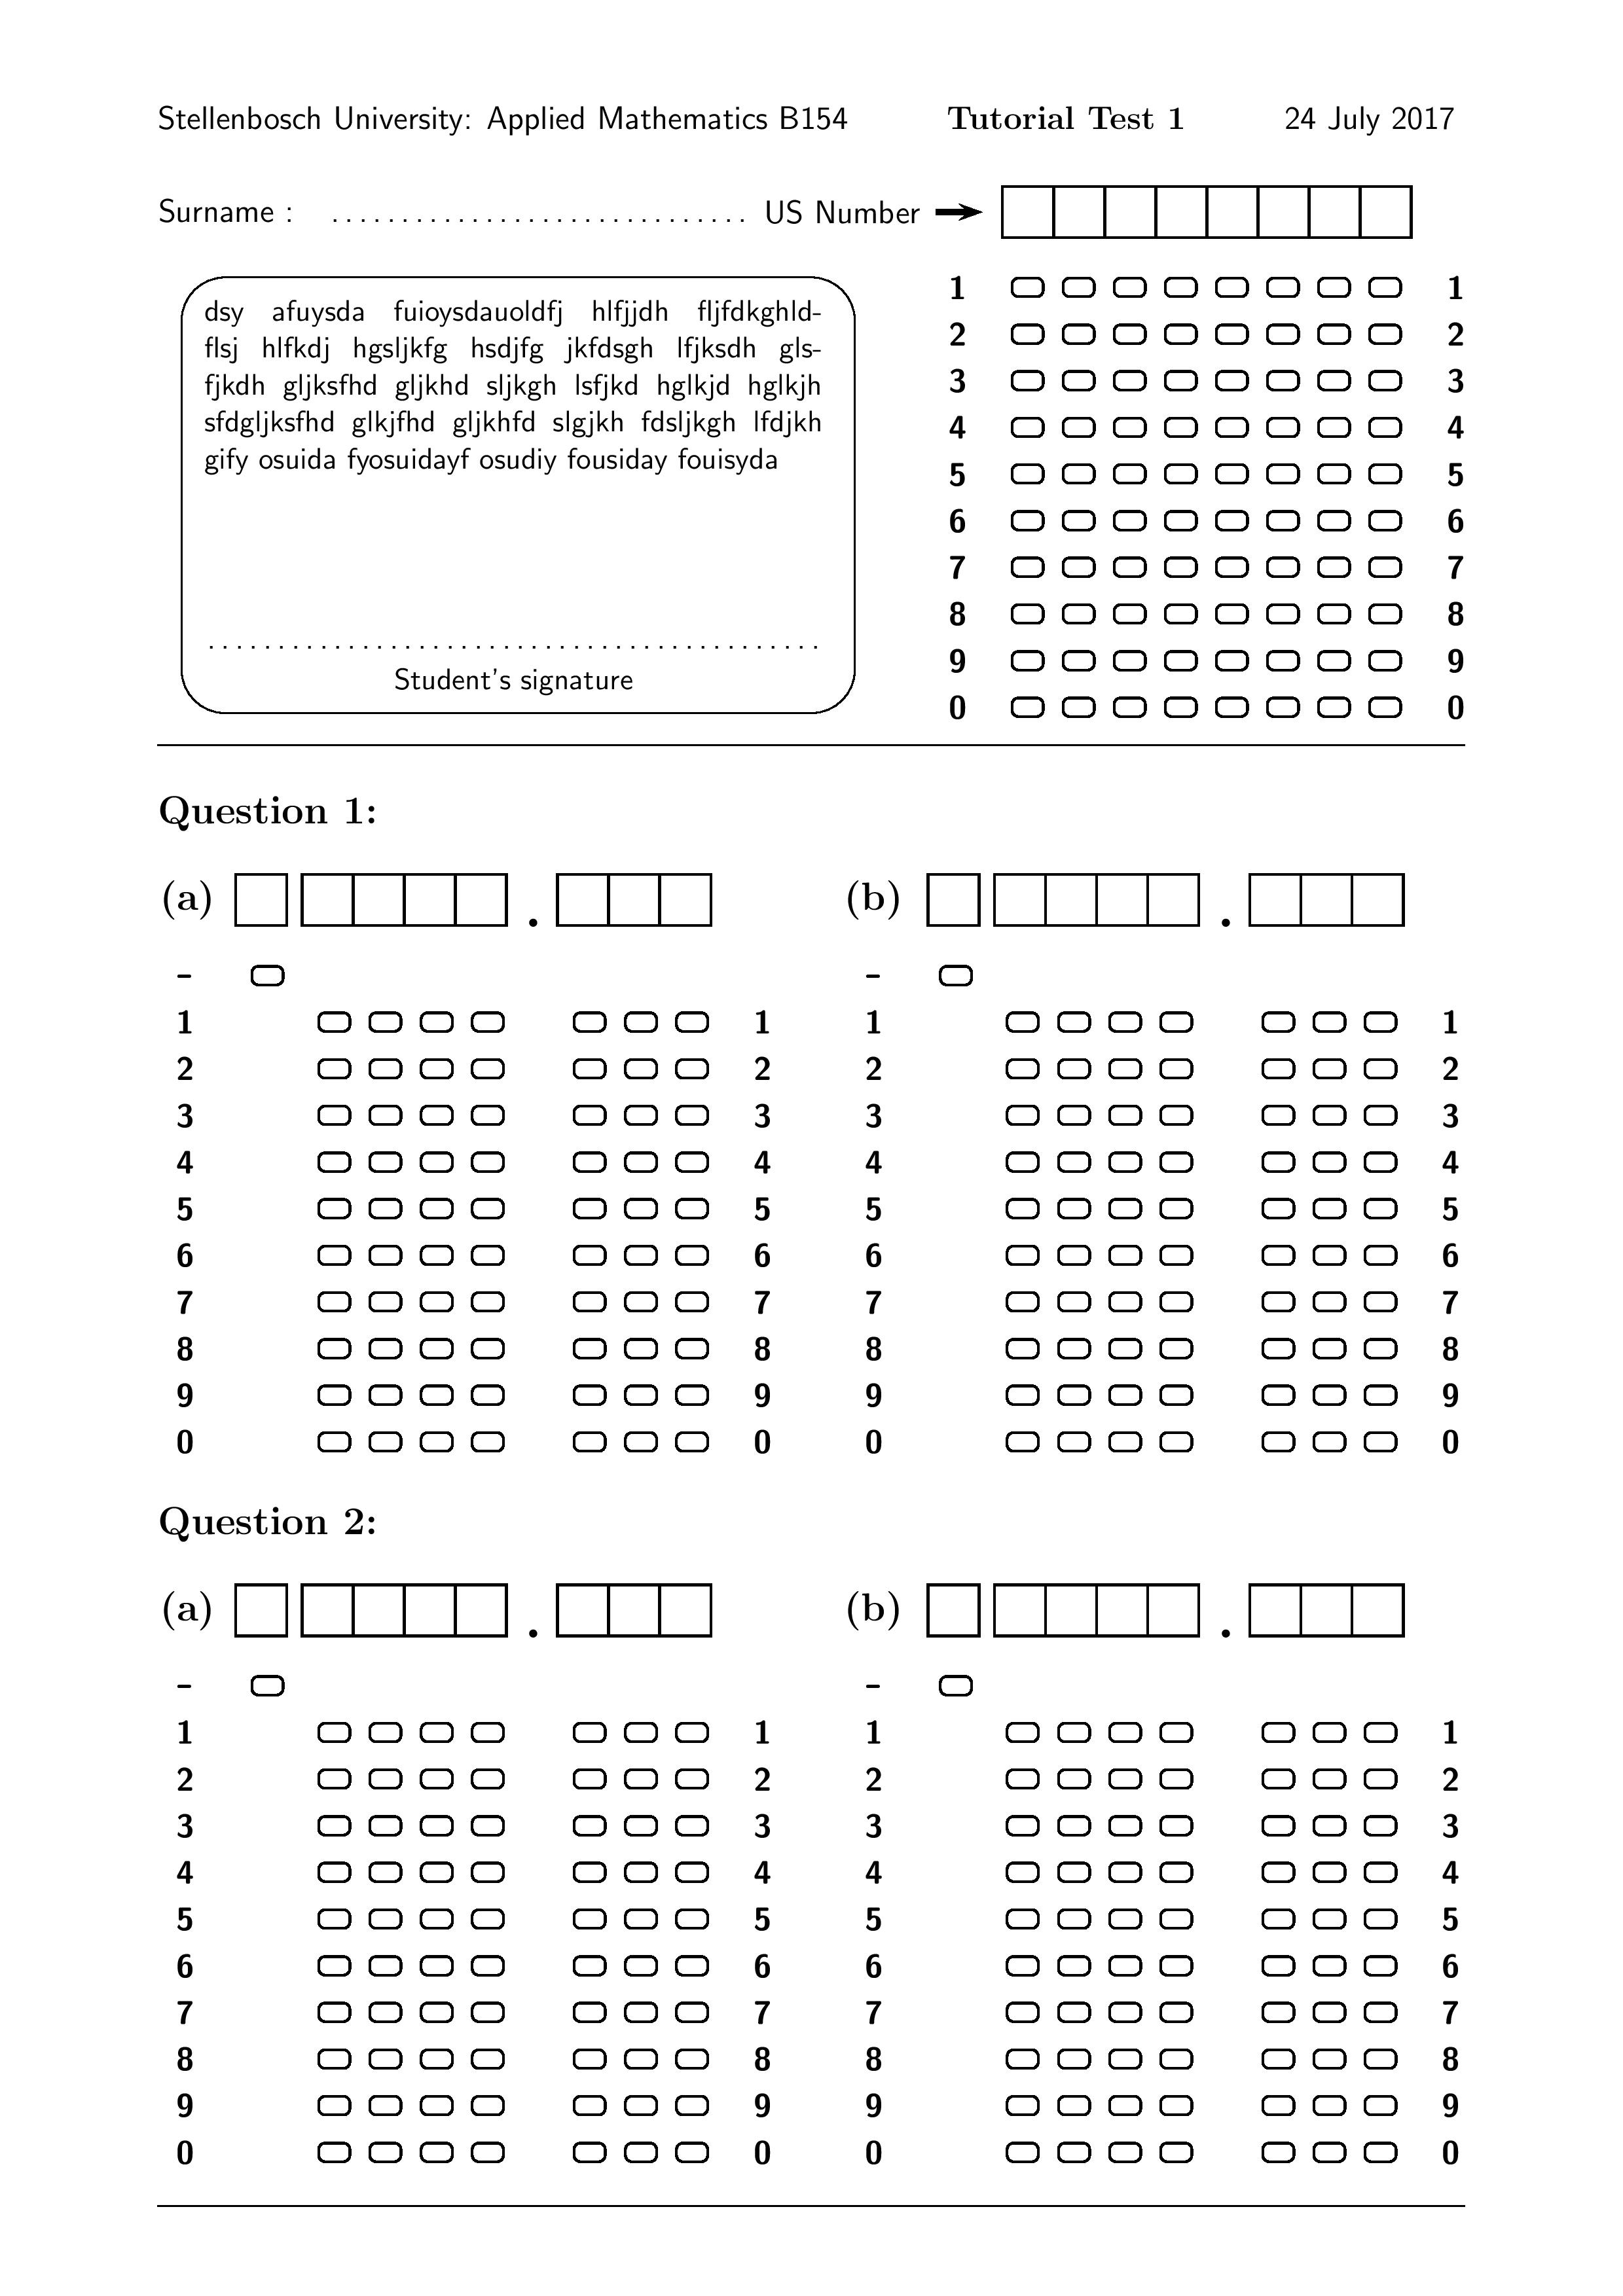
\includegraphics[width=14cm]{NumbersTemplate}\\
  \caption{Automatic grading template 1.}
  \label{fig:NumbersTemplate}
\end{figure}

\section{Project objectives}
\label{sec:Objectives}

The problem as stated in section \ref{sec:problemStatement}, is addressed by pursuing the following objectives:
\begin{enumerate}
  \item Do a \textsl{literature study} on the topics of \textsl{Image Processing},\textsl{Computer Vision} and \textsl{Character Recognition}.
  \item Develop a \textsl{software application} to enable a \textsl{user} to grade a large number (approximately 1000) scanned in student tests automatically.
  \item Do a weekly \textsl{validation experiment} with the software, by grading tutorial test for the department. The results are then used as the student's grade for that test.
  \item Use an \textsl{agile development methodology} to improving the software in parallel with the grading of weekly tests.
  \item Add additional software to allow grading of new \textsl{templates} and to increase the speed and accuracy of the software.
\end{enumerate}

The objectives are covered in different chapters in the report. Note that each objective (1--5) build on the objective(s) previously listed.

The software must also ease the use of the template for students while also providing precise and useful feedback. To do this every graded result will also include feedback on what answers the student got wrong and what the correct answers were. To increase ease of use, software is developed that provides the luxury to students to only writing down their student numbers. Thus time does not get wasted filling in the student number bubbles. This result is achieved in Chapter \ref{sec:pgmStudentNum}.

\section{Research methodology}

To complete the objectives listed in Section \ref{sec:Objectives}, a agile development methodology is used. The methodology followed comprises of five different phases:
\begin{enumerate}
\item Identify a new feature or update that needs to be implemented into the software package.
\item Do a study on the existing methods to implement this new software.
\item Implement and integrate the new software with the current knowledge of the solution.
\item Test the software and observe if it is working as planned.
\item If the software is not working as planned, revisit steps 2-4 until the new software is working.
\item Use version control, for example Git, to save the latest version of the software.
\end{enumerate}

The structure and graphical overview of the software, is presented next.

(Vra prof of my wiskude reg is oor hoe die PGM stelsel werk.)

\section{Graphical overview of system}
\subsection{System overview}

When thinking about the system (for template 1), from a philosophical sense, it can fundamentally be represented with 6 information nodes. The student has certain information he/she wants to portray on the paper. This includes the 4 answers and student number he/she wants to write down. Thus those 5 nodes gives rise to the image, representing the last node. This has to be represented in a probabilistic way. This is, because the process of writing answers down and scanning the test sheet in is going to produce a different image every time a test is written, even though the same answers are intended. This graphical model is illustrated in Figure \ref{fig:systemOverview}. The unnamed blocks indicate that information processing happens in these steps. For the complete visual overview of the system, again refer to Appendix \ref{ap:systemOverview}.
\begin{figure}
  \centering
  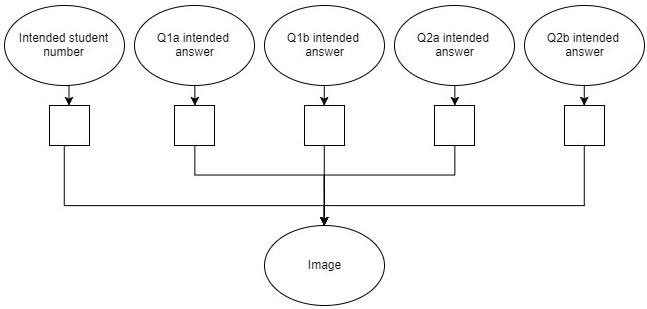
\includegraphics[width=11cm]{systemOverview}\\
  \caption{Graphical overview of the system as a whole.}
  \label{fig:systemOverview}
\end{figure}

\nomenclature[pgmAcronym]{$PGM$}{Probabilistic graphical model}

For a more detailed mathematical derivation of the entire system, refer to Appendix \ref{ap:systemOverview}.

\subsection{Graphical representation}

For this project a graphical approach is followed in representing the software developed. A graphical model in essence allows software to be represented as information (nodes or circles) and relationships (directed arrows). The directions of the arrows represents what information causes other information to be created, thus given a parent to offspring interpretation). An example of such a graph can again be seen in Figure \ref{fig:systemOverview}. This allows intuitive reasoning about how the system should operate. An observation is always made in the form of an image and then the system is tasked with predicting what the written answers are. Due to the probabilistic nature of the system a probabilistic component is also needed in this graphical models. Thus a probabilistic graphical model (PGM) is used.

A PGM is in essence the same as a general graphical model. The only difference is that now the information and relationships between information bubbles are probabilistic and not always certain as with general logic graphical models.

A literature study is presented next on methods currently used by existing automatic test grading systems. This will describe in the next chapter.